The WR technology \cite{Wlostowski2011} is an international, collaborative
project started at CERN in 2009, and then joined by other laboratories and
companies. It was born as replacement technology for the timing system at CERN,
but thanks to its versatility, improved performance, compared to the
alternatives, and open nature of the project, it was quickly adopted by other
scientific institutions.  There is also interest by some private companies, 
such as Creotech or Seven Solutions, for extending the use of WR in the 
industrial world. Some examples of that effort are the projects WR-SYNTEF 
\cite{web:creotech_projects} and IFMIF/EVEDA \cite{web:seven_projects}. 

The WR protocol extends PTPv2 with extra messages and has been proposed to be
included in the new PTP release (PTPv3) as High Accuracy (HA) profile
\cite{wr:maciej-ptpv3-standard} . Its main goal is to provide a synchronisation
accuracy better than 1 ns and precision in the scale of picoseconds. The major
improvements introduced in the WR protocol address weak aspects of the PTPv2:
the limitation in the phase difference measurements to one period of the system
clock; and the assumption of symmetry between the transmission and reception
paths. It inherently performs self-calibration over optical fibre links and it
is capable of distributing time to a very large number of devices with very
small degradation. Nevertheless, this technology in the origin was not designed
to address large distances and the inclusion of monitoring and dependable
mechanisms in the nodes. Although SKA is working on improving both issues, we
particularly focus on this contribution on presenting a new platform capable to
disseminate the PPS signal incorporating flexibility and dependability features.  

The WR synchronisation mechanisms include the following elements:

\begin{itemize}
    
\item Frequency synchronisation (syntonization): The recovered clock from the 
physical layer (L1) of the Open Systems Interconnection model (OSI) is used by 
the WR logic to syntonize the local oscillator. That means that all the WR 
network run syntonized with the main clock reference.

\item Phase synchronisation: Thanks to the syntonization, the one-cicle time 
resolution limitation is resolved via the use of the Dual Mixed Time Difference 
method (DMTD). A digital implementation of that \ref{Moreira2011} is used to 
achieve sub-picosecond resolution when measuring phase difference between the 
local oscillator and the recovered one from the upwards node.

\item Time synchronisation: It is implemented by an enhanced version of the 
PTPv2 protocol and provides a global notion of time to the entire network. WR 
also takes into account the asymmetries in the propagation time due to
the utilisation of different wavelengths in the same fibre link improving the 
accuracy of standard PTP protocol. 
\end{itemize}

WR implements mechanisms to ensure deterministic and reliable data transfer
between a thousand of nodes connected with  optical fibre links up to 10 km.
However, it can easily be extended up to a hundred of km without the need of 
optical amplification. This is easily achieved using transceivers for long 
distances commercially available.

\subsection{Network topology} \label{subsec:wr-net}

A typical WR network presents a tree topology and is composed of three different
kind of elements: a Grandmaster (GM), several intermediate devices such as
switches and the end-nodes as shown in the Figure \ref{fig:wr_hierarchy}. The GM
is normally connected to a very stable clock such as an atomic clock or a GPS
receiver \cite{Daniluk2012}. The intermediate levels of the network disseminate
the timing packets to the final nodes, which are composed of other devices such
as WR Switches, WR-ZEN or WR Light Embedded Node (WR-LEN). These devices have
several ports and can behave as PTPv2 Boundary Clocks (BC). Moreover, they are
connected using the master-slave scheme: some ports acting as slave (upstream)
and connect to the upper layer while the others are masters (downstreams) and
they are charged of propagating the synchronisation to the next level of the
hierarchy. The nodes of the last level of the network are known as slave devices
that recover the clock signal of the link and synchronises their local
oscillators to provide synchronisation for a specific application.

In addition to the conventional tree topology of the timing networks, new
network topologies are under-study in WR to add some mechanisms to improve fault
tolerance and security currently. An example of this research is
\cite{jlgutierrez-paper-redundancy} that incorporates the Transparent Clocks
(TC) to WR protocol and allows implementing redundancy protocols such as
High-availability Seamless Redundancy (HSR) or Parallel Redundancy Protocol
(PRP) to ensure the data delivery and reception in critical applications such as
control network, real-time applications or Smart Grids among others.

\begin{figure}[H] \centering 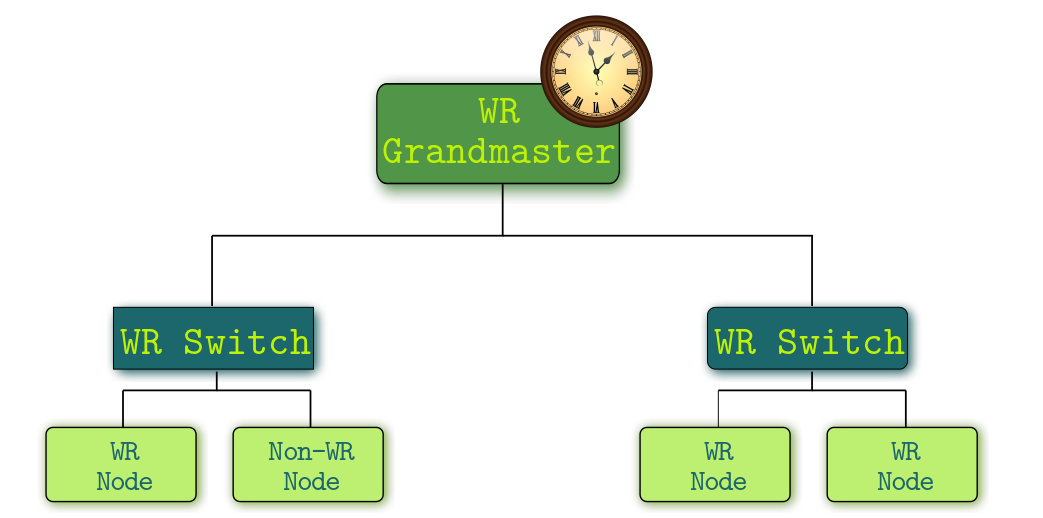
\includegraphics[scale=0.4]{img/wr_hierarchy}
	\caption{The WR network is a tree hierarchy where the root node is the
	GM that is responsible for distributing the reference time signals. The
	intermediate elements are WR Switches that acts as Gigabit Ethernet
	switches and as Boundary Clocks propagating the time signals from the
	upper layers of the network. Finally, the main purpose of the end-nodes
	is to provide timing to another specific application.}
\label{fig:wr_hierarchy} \end{figure}

\subsection{Selection of WR devices for the SKA Telescope} \label{subsec:wr-dev}

Regardless of the case of use for the WR technology, it will be needed to select
a suitable set of WR devices. Most applications distinguish two main roles
according to a typical WR network: devices which act as BC, and ones that act as
Ordinary Clocks (OC). Currently, the WRS \cite{ohwr:wrs} is the most convenient
BC among all the WR devices. 

The WRS has a total of 18 Small Form-factor Pluggable (SFP) transceivers, one 
of which can be configured as slave (upstream) and the rest as masters 
(downstream). It is also important to remark another I/O ports such as: five 
coaxial RF connectors and one management Ethernet RJ45 connector. Although 
there are other WR devices that could act as BC, the WRS is the most 
appropriate for a network with a high number of nodes, such as is the SKA 
Telescope, because of its high number of SFP slots.

The selection of the device acting as OC is not an easy task. Nowadays, there
are several platforms including the WR technology, so that, we have analysed
three devices taking into account the specific requirements of the SKA project.

Table \ref{tab:wr_devcomp} contains a comparison between the following three WR
devices: \begin{itemize} \item The Simple PCIe FMC carrier (SPEC)
			\cite{ohwr:spec} is a WR-compliant FMC carrier that
			supports low pin count (LPC) boards. It includes a
			Xilinx's Spartan-6 FPGA, an SFP connector and a PCIe
			interface. It could be used in standalone mode
			\cite{migueljl-paper-wr-spec}, but due to its limited
			computational resources, the SPEC is usually used
			connected to a host PC using the PCIe interface.  No
			coaxial RF connectors are included in the board. This is
			a major penalty because even for taking the PPS, an
			external FMC board is needed.
	
	\item The WR Light Embedded Node (LEN) \cite{sevensols:wr_len} is a
		standalone WR node whose main design principles are: an easiness
		of use and a good timing performance. It is the first WR node
		that included the extended version of the WR PTP core (WRPC)
		architecture, the WR PTP Core Dual Port (WRC2P)
		\cite{torres2016scalability}. Besides the a second WR-compliant
		Ethernet interface, the WR-LEN includes three coaxial RF
		connectors and a Ethernet RJ45 management port. Its design is
		quite similar to the SPEC board, but with some component
		upgrades, such as the FPGA (Xilinx's Artix-7).
	
	\item The WR Zynq Embedded Node (ZEN) \cite{sevensols:wr_zen} is another
		standalone WR node but with many improvements compared to the
		rest of WR nodes. As in the WR-LEN, the WR implementation
		corresponds to the WRC2P.  That enables a BC configuration as
		well as OC, or GM configurations. Design is based in a FPGA-SoC
		from Xilinx (Zynq-7000). Thanks to the dual ARM core included on
		that, the node's design is improved by the use of an Linux-like
		OS. The board main I/O connectors are: a FMC high pin count
		(HPC), two SFPs, five coaxial RF and two Ethernet RJ45. The
clocking resources include a low-noise oscillator and a flexible PLL schema.
\end{itemize}

 \begin{threeparttable}\centering \ra{1.1} \begin{tabular}{@{} lccc@{}}%\toprule
	 & \rotatebox[origin=c]{60}{SPEC} & \rotatebox[origin=c]{60}{WR-LEN}  &
	 \rotatebox[origin=c]{60}{WR-ZEN} \\ \midrule \textbf{WR-compliant}\\
	 \tab\small{+BC} & \Circle & \CIRCLE & \CIRCLE \\ \tab\small{+OC} &
	 \CIRCLE & \CIRCLE & \CIRCLE \\ \tab\small{+GM} & \LEFTcircle &
	 \LEFTcircle & \CIRCLE \\ \tab\small{+Standalone} & \LEFTcircle &
	 \CIRCLE & \CIRCLE \\
		
		\textbf{RF interfacing}\\ \tab\small{+PPS output} & \LEFTcircle
		& \CIRCLE & \CIRCLE \\ \tab\small{+RF I/O} & \Circle & \CIRCLE &
		\CIRCLE \\ \tab\small{+GM input} & \LEFTcircle & \LEFTcircle &
		\CIRCLE \\
		
		\textbf{Dev. support}\\ \tab\small{+Monitoring support} &
		\LEFTcircle & \LEFTcircle & \CIRCLE  \\ \tab\small{+Linux OS} &
		\Circle & \Circle & \CIRCLE \\ \tab\small{+Available resources}
		& \LEFTcircle & \Circle & \CIRCLE \\
		
		\textbf{Extensions}\\ \tab\small{+FMC connector} & \LEFTcircle &
 \Circle & \CIRCLE \\ \tab\small{+Redundancy} & \Circle & \LEFTcircle &
 \LEFTcircle \\ \bottomrule \end{tabular} \begin{tablenotes} \item \hfill
		 \small{\CIRCLE Fully supported; \LEFTcircle Partially
 supported; \Circle Not supported} \end{tablenotes} \caption{Comparison between
 three WR nodes.} \label{tab:wr_devcomp} \end{threeparttable}

The WR-ZEN is selected among the rest of WR nodes for the SKA Telescope because
it is most flexible platform. It is a standalone node with Linux support that
also includes enough I/O ports (RF, FMC, etc.) and improved clocking resources
looking to fulfil the timing requirements of the project.

%WR is designed to be fitted in a Field Programmable Gate Array (FPGA) device
%due to its flexibility to use in designs in a continuous development state.
%The source code is mainly written in Hardware Description Languages (HDLs) such
%as VHDL or Verilog. Moreover, there are several platforms that can implement WR
%that ensures the vendor-independent feature of WR. The most extended vendor in
%WR world is Xilinx, some examples of devices using Xilinx's FPGAs are the SPEC
%board \cite{ohwr:spec} and the WRS \cite{ohwr:wrs}. The other vendor used in WR
%is Altera. Some examples of boards could be found in \cite{cesar-altera-wr}.
%The main Intellectual Property (IP) block is the WR PTP core (WRPC) for WR
%nodes and the Real Time Subsystem (RTS) for WR switches. 

%The utilization of the previous WR-compliant nodes in the SKA system presents
%an important problem: they are based on PCIe interface cards to be plugged on
%standard computers, microTCA or VME-64 crates and therefore, a specific
%computer is necessary to provide the high level software management
%functionalities. Although most of these cards can be used on stand-alone
%operation mode, they just use a FPGA device as processing engine and this make
%very complicated to add new functionalities or standard software tools. The
%main WR node designs include a soft-microprocessor on the FPGA gateware but it
%is not enough to fully solve the problem because it requires using complex
%non-standard firmware programming tools and it normally translates on high
%time-intensive development effort and makes difficult the upgrade of the system
%firmware. We have worked with these platform in order to build a sensor network
%based on the SPEC board allowing the PC-hosted and the standalone modes
%\cite{migueljl-paper-wr-spec}.

%As a different solution, we present a new platform based on an enhanced
%technology: The WR Zynq Embedded Node (WR-ZEN) \cite{sevensols:wr_zen}. It is a
%new generation board that includes a Xilinx Zynq System-on-Chip (SoC)
%\cite{xilinx:zynq}. The Zynq SoC is composed of a FPGA and a hard ARM dual core
%microprocessor that can run an application that controls the hardware directly
%or a standard Operating System such as Linux that can host many different kind
%of processes at the same time. Moreover, the WR-ZEN allows developing gateware
%and software on the same chip, tightly integrating performance and flexibility
%thanks to the use of the co-design strategies. The WR-ZEN offers several
%advantages over the old WR-compliant nodes (WR-LEN, SPEC or SVEC) such as an
%enhanced standalone mode with a Linux system that can include high level
%software capabilities without an external PC and the new clocking circuitry
%among others. Accordingly, the WR-ZEN has been proposed to be used in the SKA
%project to implement the PPS distribution system and currently, it is being
%evaluated as a candidate solution for the SKA PPS distribution system.  

%Next sections will present the proposed system for SKA and the main WR
%contributions: WR Precision Time Protocol for clock propagation and the
%generation of PPS signal. 
